\chapter{Evaluation}
\label{ch:Evaluation}

In this chapter the prototype is evaluated in terms of its functionality and its properties.

All possible valid configurations will be generate for one use case i.e. all possible valid configurations for the forest use case.

Generate groups with preferences (explicit preferences) and configuration state (which would be for example the currently existing forest).

\section{Metric}
\label{sec:Evaluation:Metrics}

For the evaluation a metric to evaluate by is needed. The proposed metric for usage is that of satisfactions. Satisfaction will be quantified by a threshold metric. A user's preference is used to calculate a rating for each possible solution. The score will be calculated using the average of a user's rating for each characteristic that is part of the solution. The result allows that a configuration can be compared to all other configurations and ranked according to the percentage of configurations that it beats. 50\% is used as base line and the parameter this metric accepts is something that will be called satisfaction mean distance $smd$. The users counting as satisfied with a solution find the solution to be better than $50\% + smd$ of all possible solutions. Respectively a solution that ranks among the lowest scored $50\% - smd$ is classified as unsatisfied.

\section{Questions to Answer During the Evaluation}
\label{sec:Evaluation:Questions}

\begin{itemize}
    \item Main question: How does the satisfaction with a group decision, guided by a the recommender, differ from the decision of a single decision maker, who does not take the other group member's opinion into account?
    \item How many group members are satisfied with the group decision on average?
    %\item Is the recommender fair, i.e. no user type is always worse off than others? (Just uses groupe preferences)
    \item How does the amount of stored finished configurations relate to recommendation satisfaction?
\end{itemize}

\section{Effect of Stored Finished Configurations}
\label{sec:Evaluation:EffectFinishedConfiguration}

When evaluating just a subset of stored finished configurations it is important to avoid outliers. This is the reason why a process inspired by cross validation is used. The configuration database is randomly ordered and sliced into sub databases of the needed size. As an example, if the evaluated stored data size is 20, a configuration database containing 100 configurations is split into five sub databases of size 20. Now the evaluation is done on each of the sub databases and as a result the average is taken.

\section{Use Case}
\label{sec:Evaluation:UseCase}

To evaluate data a given use case is needed. In this thesis a forestry use case is evaluated. This is a use case with four stakeholders. \autoref{fig:Concept:ForestExample} already presented the attributes and characteristics used in this use case but an extension is needed to fully show the whole use case. Namely rules of non valid configurations. The constraints for this use case are listed in not with form in \autoref{tab:Evaluation:UseCase}. 

\begin{table}
    \begin{center}
        \begin{tabular}{r|l}
            & not with (either of the listed) \\
            \hline
            $(\textit{indigenous}, \text{moderate})$   & $(\textit{resilient}, \text{high})$ \\
            \hline
            $(\textit{indigenous}, \text{high})$   & $(\textit{resilient}, \text{high}), (\textit{usable}, \text{moderate}), (\textit{usable}, \text{high}),$ \\
            & $(\textit{quantity}, \text{high}), (\textit{price}, \text{low})$ \\
            \hline 
            $(\textit{resilient}, \text{moderate})$   & $(\textit{usable}, \text{high})$ \\
            \hline
            $(\textit{resilient}, \text{high})$   & $(\textit{usable}, \text{high}), (\textit{usable}, \text{moderate}), (\textit{quantity}, \text{high}),$ \\
            & $(\textit{price}, \text{moderate}), (\textit{price}, \text{low})$ \\
            \hline
            $(\textit{usable}, \text{low})$ & $(\textit{quantity}, \text{high}), (\textit{price}, \text{moderate}), (\textit{price}, \text{low})$\\
            \hline
            $(\textit{usable}, \text{high})$ & $(\textit{accessebility}, \text{high})$\\
            \hline
            $(\textit{effort}, \text{manual})$ & $(\textit{quantity}, \text{high}), (\textit{price}, \text{low}), (\textit{price}, \text{moderate})$\\
            \hline
            $(\textit{effort}, \text{harvester})$ & $(\textit{accessebility}, \text{high}), (\textit{accessebility}, \text{moderate})$\\
            \hline
            $(\textit{effort}, \text{autonomous})$ & $(\textit{accessebility}, \text{high}), (\textit{accessebility}, \text{moderate})$\\
            \hline
            $(\textit{quantity}, \text{low})$ & $(\textit{price}, \text{low}), (\textit{price}, \text{moderate})$\\
            \hline
            $(\textit{quantity}, \text{moderate})$ & $(\textit{price}, \text{low}), (\textit{price}, \text{moderate})$\\
            \hline
            $(\textit{quantity}, \text{high})$ & $(\textit{accessebility}, \text{high}), (\textit{accessebility}, \text{moderate})$\\
            \hline
        \end{tabular}
        \caption{Constrains in not with form for the forest use case.}
        \label{tab:Evaluation:UseCase}
    \end{center}
\end{table}

\section{Generating Data}
\label{sec:Evaluation:GeneratingGroups}

The whole process explained in this section is visualized in \autoref{fig:Evaluation:GeneratingDataProcess}.

\begin{figure}
    \centering
    \includegraphics[width=1\textwidth]{./figures/60_evaluation/bpmn_evaluation_input_data_generation.pdf}
    \caption{The process used for generating data for the evaluation.}
    \label{fig:Evaluation:GeneratingDataProcess}
\end{figure}

\subsection{Generating Unfinished Configurations}

Unfinished configurations are generated using all finished configurations and taking a subset of the contained characteristics. This way all generated configurations will be valid and lead to valid solutions. For the results that are presented in this chapter around $\frac{1}{7} \approx 15\%$ of characteristics is kept.

\todo[inline]{why this paramter, elalobrate on that}

\subsection{Generating Preferences}

For the forest use case, the idea is that there are multiple types of user profiles. Each group profile is represented by a neutral, negative or positive attitude to an attribute value. Now during data generation the attitude is converted to a preference using a normal distribution. \autoref{fig:Evaluation:DataGeneration} shows how the user profile can be converted to preferences.

\pgfplotsset{height=5cm,width=\textwidth,compat=1.8}
\pgfmathdeclarefunction{gauss}{2}{%
  \pgfmathparse{1/(#2*sqrt(2*pi))*exp(-((x-#1)^2)/(2*#2^2))}%
}
\begin{figure}
    \begin{tikzpicture}
        \begin{axis}[
            every axis plot post/.append style={
                mark=none, domain=0:1, samples=50, smooth
            },
            axis x line*=bottom,
            xmin=0,
            xmax=1,
            ymin=0.1,
            xticklabel style={
                /pgf/number format/precision=3,
            },
            xtick={0,0.25, 0.5, 0.75,1},
            hide y axis]
          \addplot [draw=red][very thick] {gauss(0.25,0.1)} node[text=red][above,pos=0.5] {negative};
          \addplot [draw=blue][very thick] {gauss(0.5,0.05)} node[text=blue][above,pos=0.48] {neutral};
          \addplot [draw=green!60!black][very thick] {gauss(0.75,0.1)} node[text=green!60!black][above,pos=0.5] {positive};
        \end{axis}
        \end{tikzpicture}
 \caption{Distribution of preferences for a user type.}
\label{fig:Evaluation:DataGeneration}
\end{figure}

These user profiles can be used to generate rather homogenous groups but also to create groups that have interests that are more conflicting. The following group types are generated:

\begin{itemize}
    \item random groups (preferences are uniformly random)
    \item heterogeneous groups (people adhere to one preference profile like forest owner, athlete, consumer, environmentalist)
    \item homogeneous groups (only one preference profile for all group members which in this evaluation is the forest owner)
\end{itemize}

\todo[inline]{explain preference profiles}

\section{Hypothesis}
\label{sec:Evaluation:Scenario}

\section{Results}
\label{sec:Evaluation:Results}

\subsection{Choosing Happiness and Unhappiness Parameter}

Results for happiness increase will vary depending on the chosen $smd$ value. This is to be expected because if it is set to low, the number of people that are happy with the decision of an individual will increase. An increase in amount of happiness means, that there is less people that can additionally be made happy. In the data though even with an $smd = 5\%$, this expected effect cannot yet be seen. But it is noticeable that the amount of people happy with the individual decision is decreasing with an increased $smd$. If $smd$ is set too high the group compromise will cause less people to be satisfied. This is because with the individual decision there will be always one person that is perfectly happy. Clearly this has the effect that choosing an $smd$ that is too high the decision maker will be satisfied with her own decision but no one else will. Additionally no one of the group will be happy with the group decision. Therefore it is expected, that with a high $smd$ the change in happiness will reach a value of negative one. The data shows these effects already with an $smd$ of $25$ where across the board all scoring functions result in a happiness decrease for the group (when looking at heterogeneous groups) but they don't reach levels of minus one in the tested range ($smd \in [5,35]$).

Surprisingly, all tested values for $smd \in [5,35]$ resulted in a decrease of unhappiness. But as expected the total number of unhappy decreased with an increase of the $smd$, as was observable already with happiness.

\missingfigure{Figure showing happiness and unhappiness with individual decision in relation to smd}


\subsection{Analysing Data}

In this section results for heterogeneous groups, random groups and homogenous groups, based on the forest use case, are shown. \autoref{fig:Evaluation:HeterogenousGroupIncrease} and \autoref{fig:Evaluation:HeterogenousGroupTotal} show results for heterogeneous groups. \autoref{fig:Evaluation:RandomGroupIncrease}, \autoref{fig:Evaluation:RandomGroupTotal} shows the results for random groups and \autoref{fig:Evaluation:HomogenousGroupIncrease}, \autoref{fig:Evaluation:HomogenousGroupTotal} show the results for homogenous groups.

The first thing that is noticed when analysing the data is that with homogenous groups the recommender does not have any benefit to an individual choosing based on their own preferences. This is most likely due to all individuals being already happy with the individual decisions. This is an effect that was noticed even when a higher $smd$ was chosen. Here we notice that the effect of not having many configurations in the store does decrease hapiness by a large amount.

When looking at results for random and heterogeneous groups the happiness level with an individual decision is much lower than individual decisions in homogenous groups. This finding is expected as random and homogenous groups are more diverse therefore opposing interest will be visible in these.

All scoring functions are similarly good in decreasing unhappiness. However the results differ when looking at happiness, Here least misery performs abysmal compared to the other scoring functions. In \autoref{fig:Evaluation:HeterogenousGroupIncrease} it results even in a hapiness reduction whereby multiplication and best average increase it. Overall multiplication seems to perform the best in most scenarios. This confirms findings in expirments with real people as described by \citeauthor{Masthoff2015} \cite[p. 755f]{Masthoff2015}.

The influence of stored configurations on performance can clearly be seen but the relationship does not seem to be linear. Therefore with already just a limited amount of stored finished configurations the recommender can increase happiness and decrease unhappiness. With 33\% of the stored configurations, the happiness increase is about 50\% to 75\% compared to using all stored finished configurations.



\begin{figure}
    \centering
    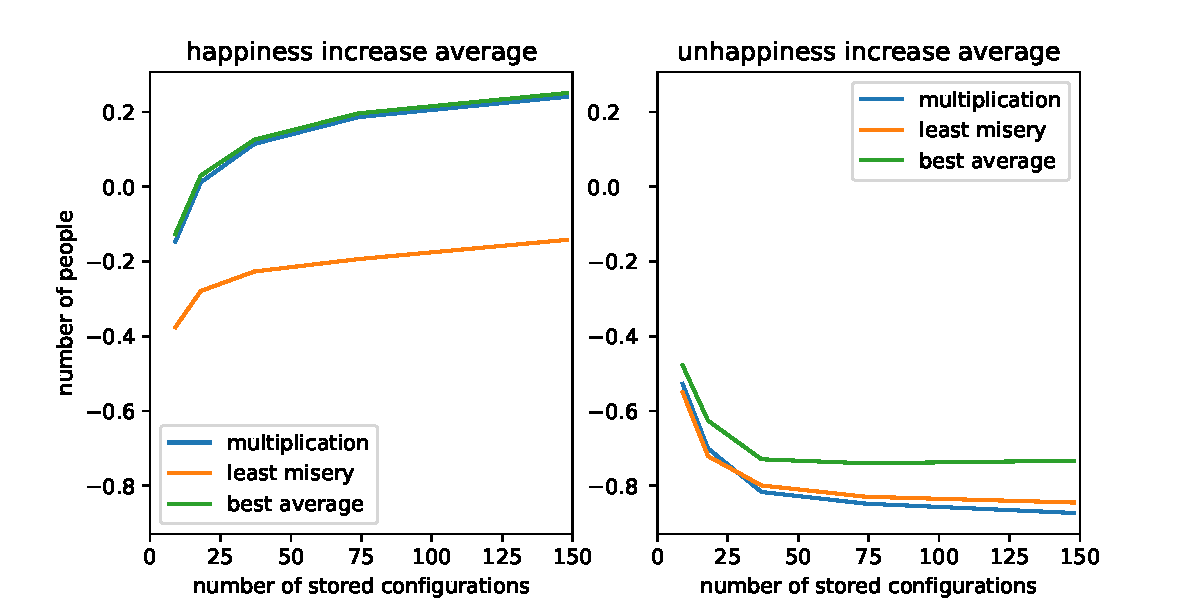
\includegraphics[width=1\textwidth]{./figures/60_evaluation/heterogeneous_happy_unhappy_increase_amount-1000_smd-15.pdf}
    \caption{The average happiness and unhappiness increase for \textbf{heterogeneous} groups consisting of four members with $smd=15\%$.}
    \label{fig:Evaluation:HeterogenousGroupIncrease}
\end{figure}

\begin{figure}
    \centering
    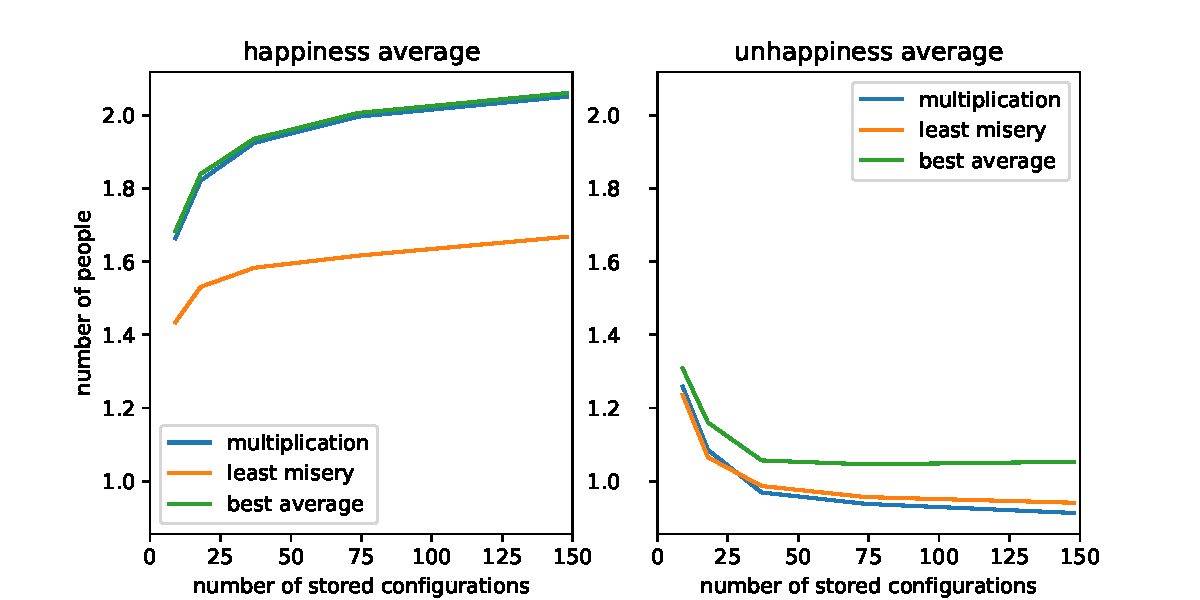
\includegraphics[width=1\textwidth]{./figures/60_evaluation/heterogeneous_happy_unhappy_total_group_amount-1000_smd-15.pdf}
    \caption{The average happiness and unhappiness for \textbf{heterogeneous} groups consisting of four members with $smd=15\%$.}
    \label{fig:Evaluation:HeterogenousGroupTotal}
\end{figure}

\begin{figure}
    \centering
    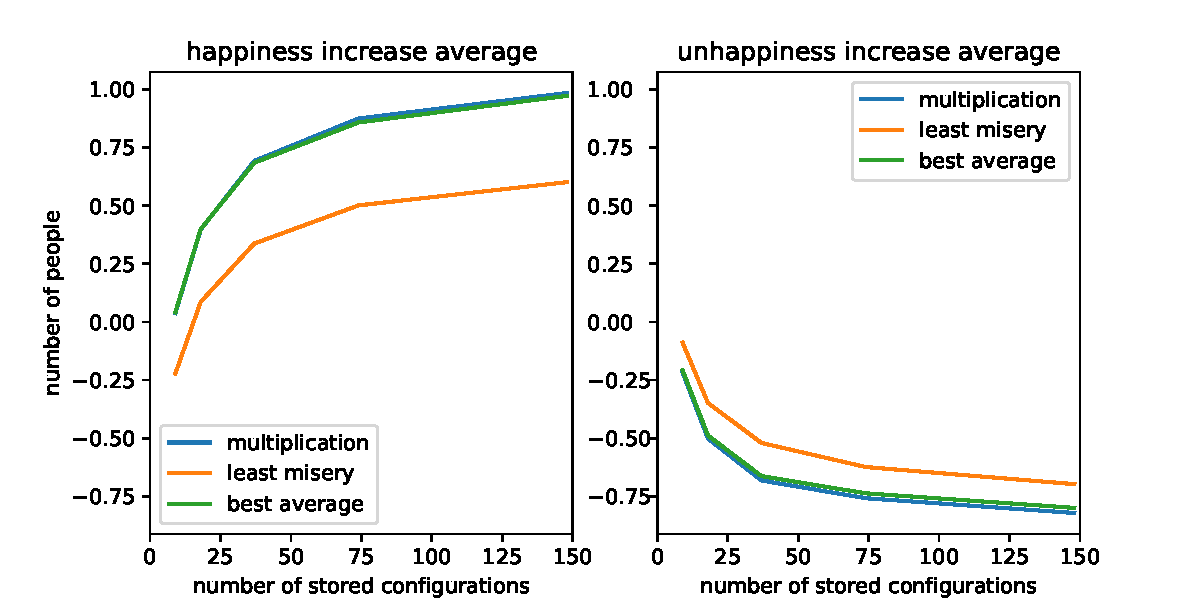
\includegraphics[width=1\textwidth]{./figures/60_evaluation/random_happy_unhappy_increase_amount-1000_smd-15.pdf}
    \caption{The average happiness and unhappiness increase for a \textbf{random} groups consisting of four members with $smd=15\%$.}
    \label{fig:Evaluation:RandomGroupIncrease}
\end{figure}

\begin{figure}
    \centering
    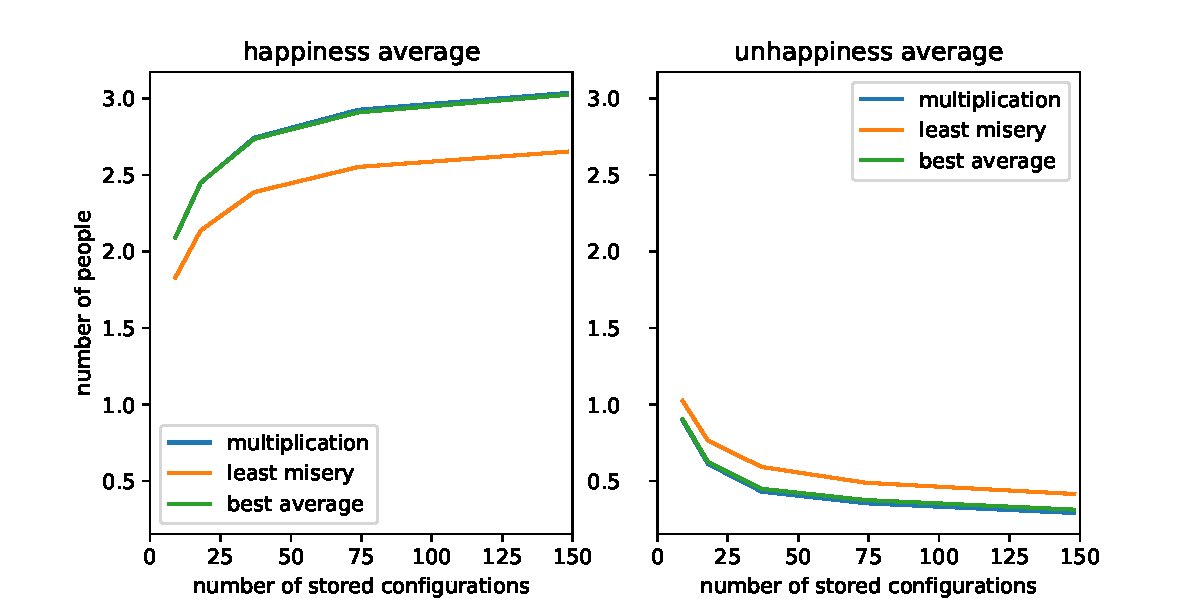
\includegraphics[width=1\textwidth]{./figures/60_evaluation/random_happy_unhappy_total_group_amount-1000_smd-15.pdf}
    \caption{The average happiness and unhappiness for \textbf{random} groups consisting of four members with $smd=15\%$.}
    \label{fig:Evaluation:RandomGroupTotal}
\end{figure}


\begin{figure}
    \centering
    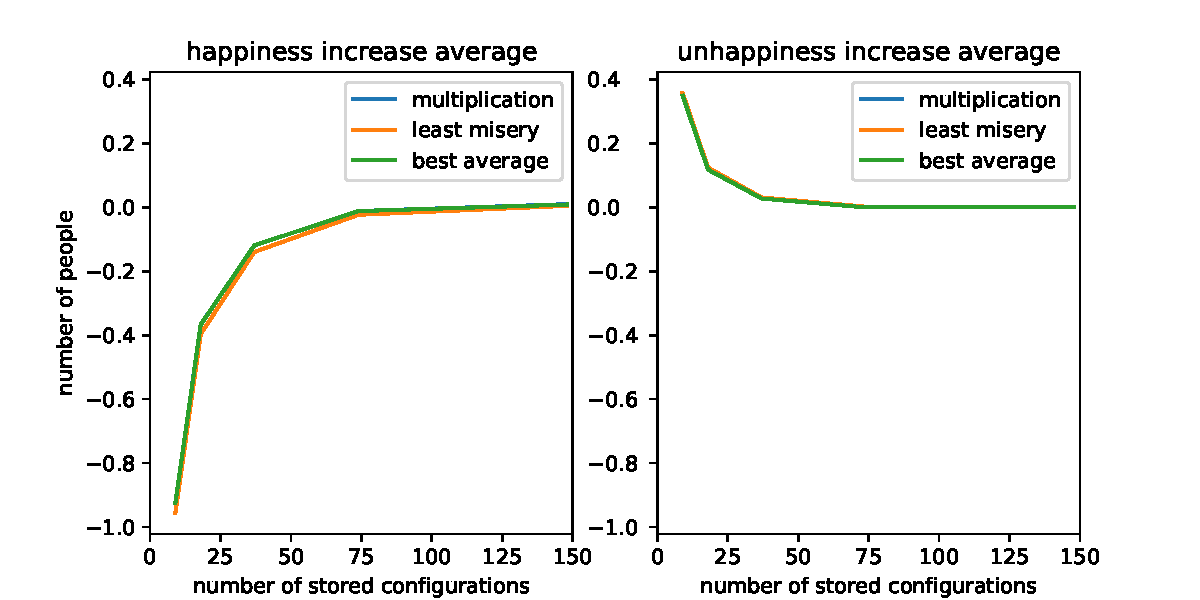
\includegraphics[width=1\textwidth]{./figures/60_evaluation/homogenous_happy_unhappy_increase_amount-1000_smd-15.pdf}
    \caption{The average happiness and unhappiness increase for a \textbf{homogenous} groups consisting of four members with $smd=15\%$.}
    \label{fig:Evaluation:HomogenousGroupIncrease}
\end{figure}

\begin{figure}
    \centering
    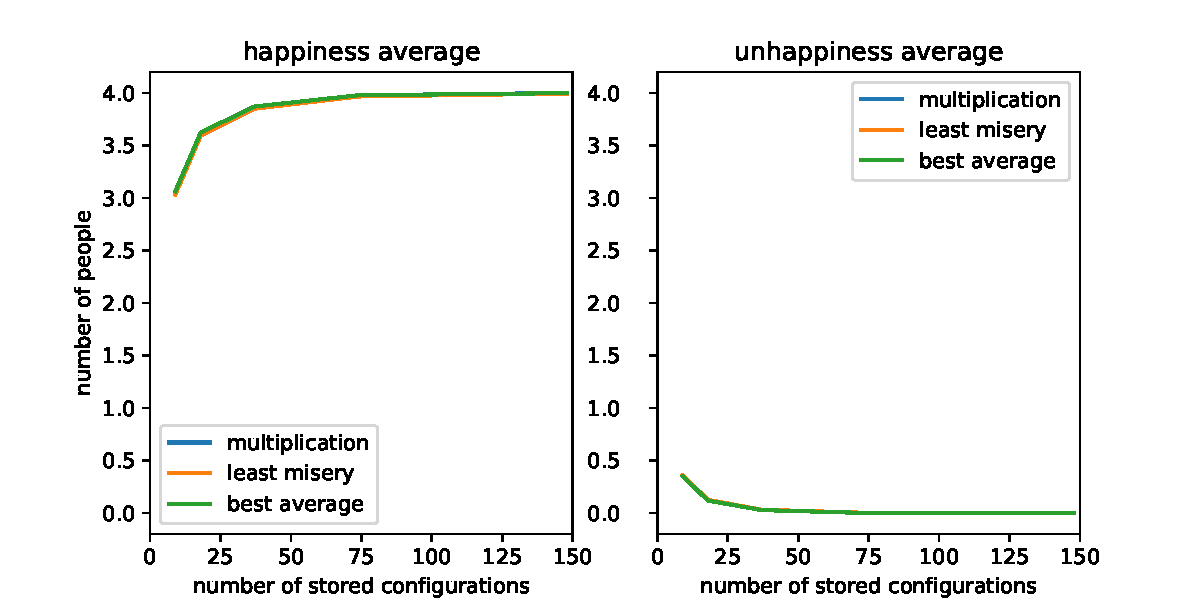
\includegraphics[width=1\textwidth]{./figures/60_evaluation/homogenous_happy_unhappy_total_group_amount-1000_smd-15.pdf}
    \caption{The average happiness and unhappiness for \textbf{homogenous} groups consisting of four members with $smd=15\%$.}
    \label{fig:Evaluation:HomogenousGroupTotal}
\end{figure}